\hypertarget{the-equation}{%
\section{The equation}\label{the-equation}}

Literature AGB yields generally have the following properties:

\begin{itemize}
\tightlist
\item
  a peak yield at mass between 2 and \(3\,M_\odot\)
\item
  asymmetric peak
\item
  near zero yield at both \(1\,M_\odot\) and \(8\,M_\odot\)
\item
  total yield with decreases with metallicity
\item
  peak mass which increases with metallicity
\item
  negative yields at lowest and highest masses at high metallicity
\end{itemize}

As a simple working model, we use a piecewise cubic spline in mass and
an independent linear relationship in log-metallicity. Our parameters
are

\begin{itemize}
\tightlist
\item
  \(m_0\)
\item
  \(\delta m_+\)
\item
  \(\delta m_-\)
\item
  \(\zeta = dy/dz\)
\item
  \(y_1\), the total yield at solar metallicity
\item
  \(y_0\), the (negative) low-mass yield
\item
  \(y_2\), the (negative) upper-intermediate-mass yield
\end{itemize}

The piecewise is defined to have a maximum at \(m_0\) and minimums at
the end points \(m_-\) and \(m_+\). The function becomes constant
outside of this range with (optionally) negative yields.

And the resulting equation (excepting a prefactor)

\[
y(m) = \begin{cases}
y_0 & m < m_- \\
y_0 + (y_1 - y_0) \left(3 (\frac{m - m_-}{m_0 - m_-})^2 - 
2 (\frac{m-m_-}{m_0 - m_-})^3\right) & m_- < m < m_0 \\
y_1 + (y_2 - y_1) \left(3 (\frac{m - m_0}{m_+ - m_0})^2 - 
2 (\frac{m-m_0}{m_+ - m_0})^3\right) & m_0 < m < m_+ \\
y_2 & m_+ > m
\end{cases}
\]

For the full equation, we take the above functional form multiplied by a
metallicity dependent term, so \[
y_{\rm C}^{\rm AGB}(m, Z) = \frac{y(m) \left[y_1 + \zeta \log_{10}(Z/Z_\odot) \right]}{\int_1^8 m\,y(m)\,{\rm IMF}(m)\;dm}
\]

\hypertarget{comparison-to-existing-models}{%
\subsection{Comparison to existing
models}\label{comparison-to-existing-models}}

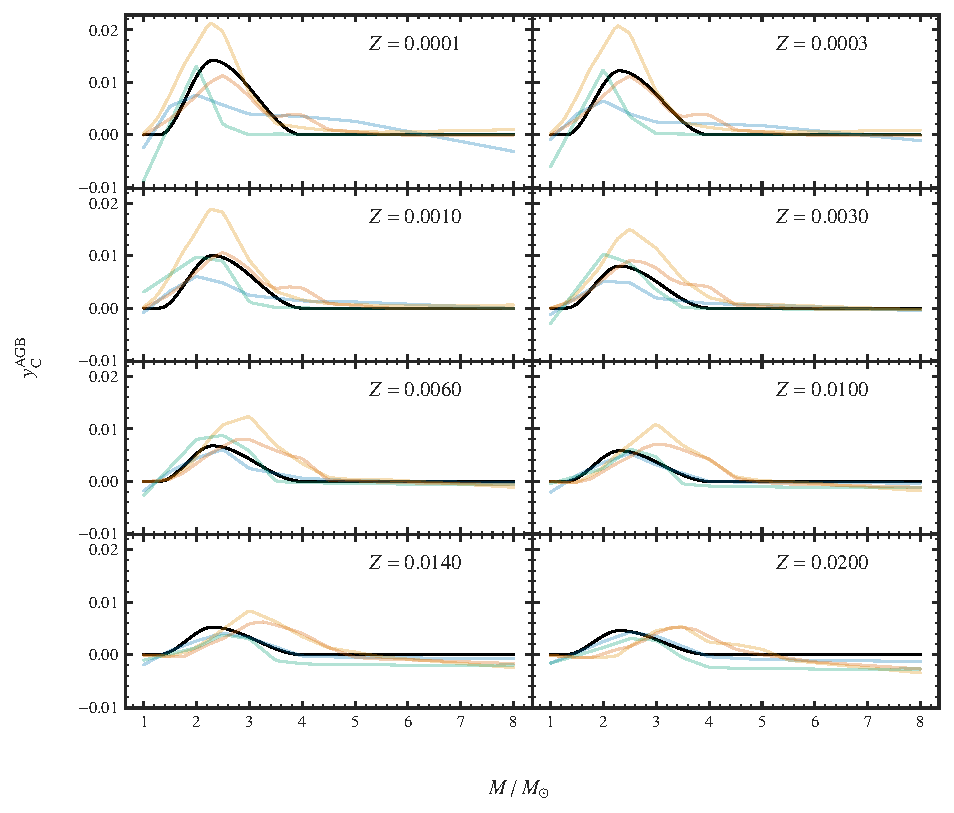
\includegraphics{figures/analytic_vs_studies_agb.pdf} A comparison
between the analytic yield model and the literature models. The AGB
IMF-integrated yield is plotted for each model as a function of mass.
Each panel displays the models at a different metallicity. As the AGB
literature models qualitatively agree, the analytic model's asymmetric
piecewise yield with a linear metallicity dependence reproduces the
qualitative behavior of the yields within the range spanned by the
models.

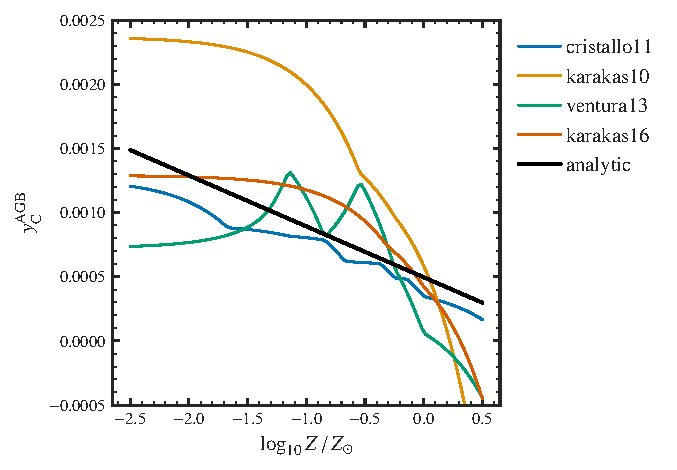
\includegraphics{figures/agb_ana_vs_z.pdf}\\
The metallicity dependence of four literature models and the analytic
AGB yield. The linear approximation is adequate since most models have
approximately linear metallicity dependence at solar \(Z\) and are
monotonic.

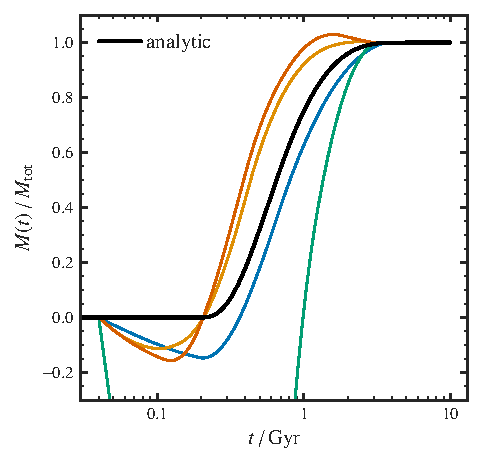
\includegraphics{figures/agb_ana_dtd.pdf}\\
The DTD of the same literature models and out analytic model. The
analytic model sits within the DTDs of all of the literature models with
the same qualitative shape. However, without the negative low and high
mass yields, the analytic model does not exhibit the overshoot at the
beginning and ends.

\hypertarget{effects-of-alternate-parameters}{%
\section{Effects of alternate
parameters}\label{effects-of-alternate-parameters}}

\hypertarget{metallicity-dependence}{%
\subsection{Metallicity dependence}\label{metallicity-dependence}}

Interestingly, the metallicity dependence of AGB yields does matter.
Increasing the metallicity dependence ``flattens'' the caafe
relationship. While we do only select one metallicity, because of the
delay time of AGB yields, the higher Mg/Fe stars, which are formed with
a rapidly declining SFH, reach higher metallicities faster. This means
that the AGB progeneters are at lower metallicity than in regions where
Mg/Fe is lower. As AGB yields are predicted to have a negative
metallicity dependence, the resulting trends are flattened.

We also note that the metallicity dependence of AGB yields is directly
degenerate with the metallicity dependence of CCSNe in caah as this is
mostlhy sensitive to the combined metallicity dependence of
IMF-integrated C yields.

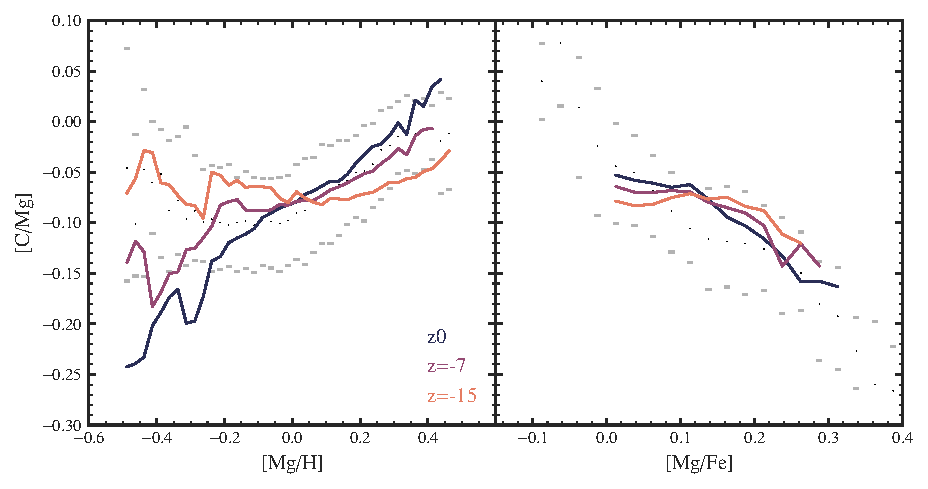
\includegraphics{figures/agb_z_dependence.pdf}\\
Each line plots a model with a different metallicity dependence. As the
metallicity dependence is increased (from z0 to z-15), the model is less
steep in caafe.

\hypertarget{mass-distribution}{%
\subsection{Mass distribution}\label{mass-distribution}}

The masses which are important for AGB C production furthermore
complicate results. When only upper intermediate mass stars produce C,
the AGB componet is produced more quickly, resulting in a flatter caafe,
similar to a higher CCSNe C fraction.

One way to conceptualize the caafe diagram is as a comparison between
the Fe and C DTDs. As this diagram is selected in metallicity, the stars
should trace out the shape of a single stellar population born at the
target metallicity -0.1. As Fe and C are produced, the track moves from
bottom right (low Fe and C) to top left (higher Fe and C) with a shape
dependent on the timescales for each process. When AGB C is weighted
heavily towards low mass stars \(\sim 1\,M_\odot\), then the DTD for AGB
is slower than Fe, resulting in a curve which bends up. On the other
hand, if the masses are weighted towards higher mass stars, then the DTD
instead bends down as C is produced quicker initially but slower at
large times than Fe.

As our obervations suggest either a non-monotonic or streight
relationship between Fe and C DTDs, we can conclude that C is produced
with a similar overall DTD as Fe is.

We can furthermore compare the effects of shifting the DTD. For our
example, m0.9 shifts up the mass of the DTD and m1,1 shifts down the
mass. as expected, both of these shifts have similar effects to the
previous investigation. However, bu shifting up the mass, the negative
yields at low masses in C11 results in a sharper down-turn than we would
expect.

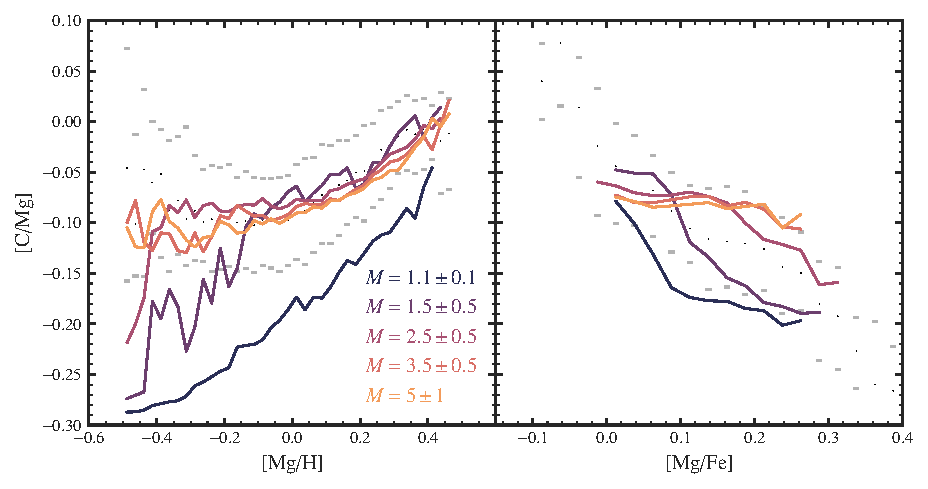
\includegraphics{figures/agb_mass.pdf}
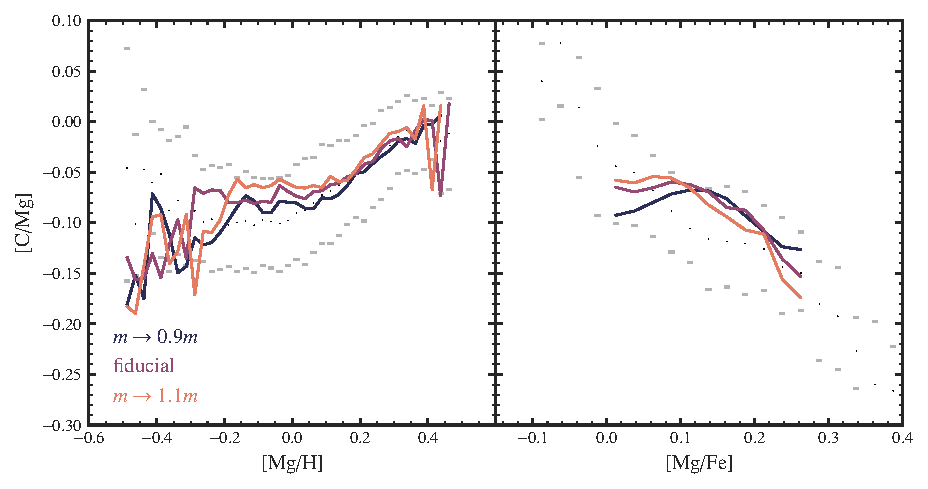
\includegraphics{figures/shift_mass.pdf}

\hypertarget{negative-yields}{%
\subsection{Negative yields}\label{negative-yields}}

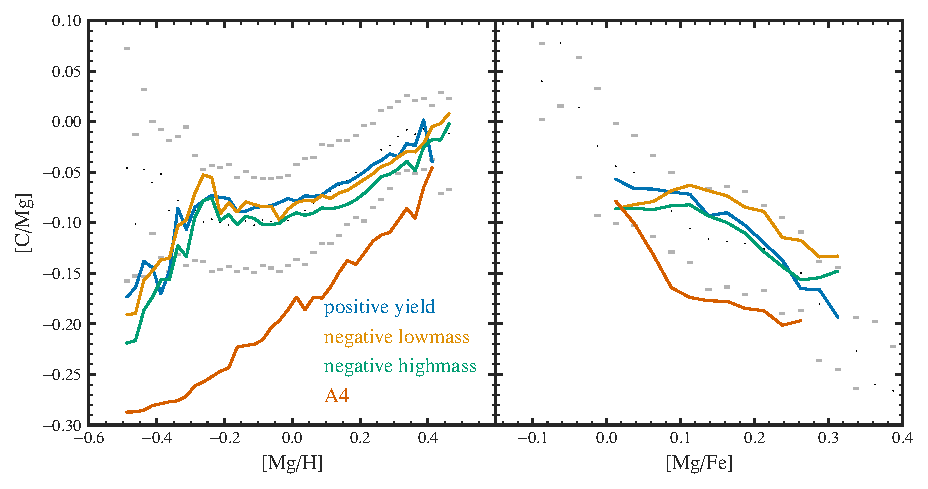
\includegraphics{figures/negative_yields.pdf} The models with negative
yields. When the low mass end of AGB stars destroy carbon, the end of
the caafe model turns down at low Mg/Fe since these are the longer lived
stars. When the high mass AGB stars destroy carbon, then only the high
Mg/Fe exhibits a dip. In either case, the effect of adding negative
yields results in a non-monotonic caafe diagram. However, we expect the
high-mass yields to be less visible as the system evolves more quickly
than at the end.

\hypertarget{alternate-sfh}{%
\subsection{Alternate SFH}\label{alternate-sfh}}

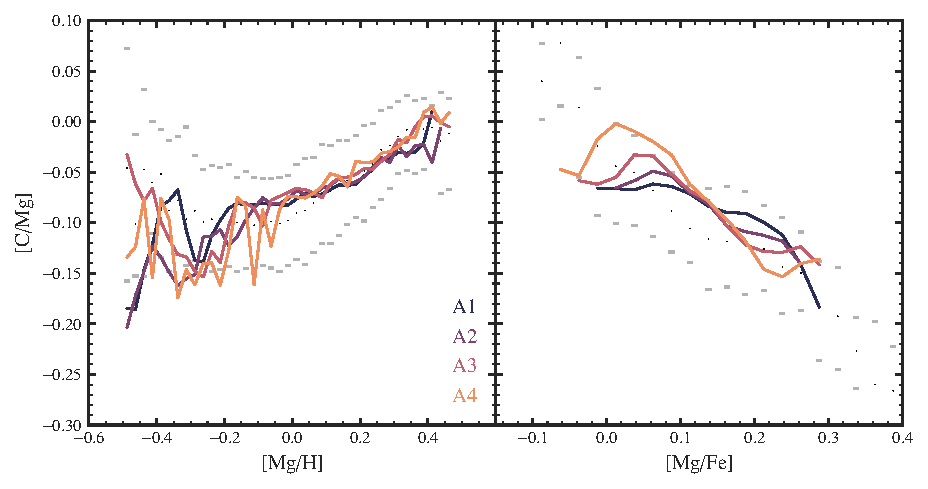
\includegraphics{figures/twoexp_strength.pdf} These are variations of
the earlyburst model in increasing strength. The effect of these two
strong bursts is to initially drop C/Mg at the beginning of the burst
and then to overhoot C/Mg at later times when Mg/Fe is closer to solar
as star formation slows down.

\hypertarget{degeneracies}{%
\section{Degeneracies}\label{degeneracies}}

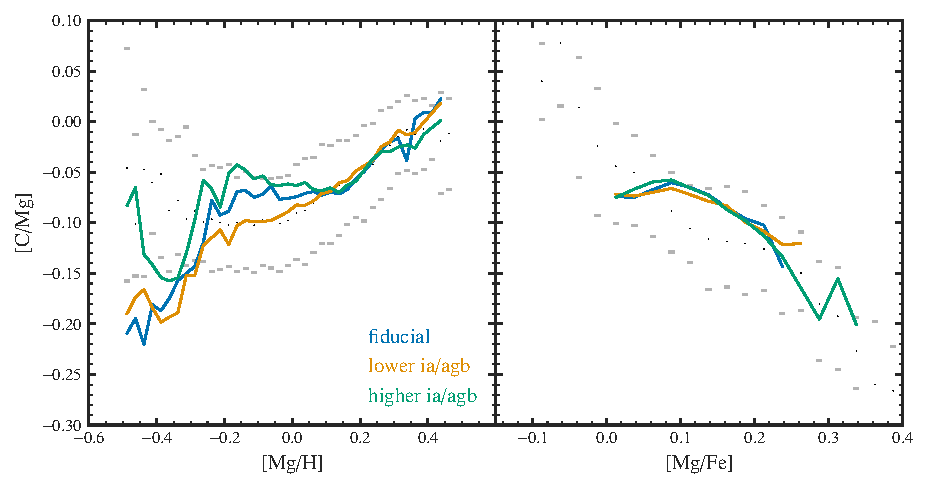
\includegraphics{figures/ia_agb_degeneracy.pdf} As the caafe depends on
both the C and Fe DTD, by adjusting both the fraction of SNeIa Fe and
AGB C simultaneously, the effects can be canceld out, so this causes an
uncertainty in the model.
